%\documentclass[letterpaper]{article}
\documentclass[12pt]{article}

\usepackage[letterpaper, portrait, margin=1in]{geometry}

\usepackage{array}	% for \newcolumntype macro
\usepackage{caption}
\usepackage{graphicx}    % This package is used for Figures
\usepackage{rotating}           % This package is used for landscape mode.
\usepackage{epsfig}
%\usepackage{comment}
\usepackage{url}
\usepackage{amsmath}
\usepackage{amssymb}
%\usepackage{cite}
\usepackage{float}
\usepackage{hyperref}
\usepackage{subfig}
\usepackage{amsmath}
\usepackage{multirow}
%\usepackage[T1]{fontenc}
\usepackage[all]{nowidow}
\usepackage[table]{xcolor}
\usepackage{circuitikz}

\usepackage{listings}

%\usepackage{grffile} % can use example.0.1.png
\usepackage{tabularx}		% Fill to margin on tables, control table width
\usepackage[normalem]{ulem}			% for strike through \sout{}
\usepackage{listings} % color the code
\usepackage{color} % to define colors
\usepackage{hhline} % to manually insert a vertical line with | or #
\usepackage{multicol} % Multiple columns
%\usepackage{pgfplots} % Plotting in LaTeX
\usepackage{enumitem} % Globally change enumerate settings. Also allows for alpha/roman switch.
%\usepackage[section]{placeins}
\setlist{nosep} % or \setlist{noitemsep} to leave space around whole list
%\usetikzlibrary{arrows} % For triangular-headded arrows
%\usetikzlibrary{patterns} % for patterns
%\usepackage[thinlines]{easytable} % For simpler table commands
\hypersetup{colorlinks=true,urlcolor=blue,urlbordercolor=blue}
\newcommand{\degrees}{$^\circ$}
\newcolumntype{M}{>{\vspace*{1cm}\hfill}p{0.223\textwidth}<{\hfill\vspace*{1cm}}} % Middle aligned

\usepackage{fancyhdr} % To create headers
\pagestyle{fancy}
%\rhead{Dr. Kunz}
\newcommand{\docTitle}{Macroscopic Circuit Analysis}
\chead{PHYS 2250 \docTitle}
\begin{document}
	\section*{Purpose}
	In this lab you will use the loop rule (energy conservation), the node rule (charge/momentum conservation) and Ohm's Law to predict and measure the voltage across and current through circuit elements in different circuits.
	
	\section*{Introduction}
	In the first part of this lab you will assemble multiple different circuits. For each circuit, you will first predict and then measure the voltage and current of every resistor in the circuit.
	
	In the second part of the lab, you will devise and carry out an experiment to determine the internal resistance of the battery.
	
	
	
	\section*{Part 1: Determining the Properties of the Battery}
	Your task for part 1 of the lab is simple: devise and conduct an experiment to determine the emf $\varepsilon$ and internal resistance $r|\mathrm{int}$ of the battery. (Note: the number printed on the battery is 9 V, but the actual emf might be slightly different, depending on a number of factors including the age of the battery). Both of these values will have associated uncertainties (you can use the Python \texttt{uncertainties} package to help with this).
	
	You have at your disposal: the multimeter (which you can use as either an ammeter or a voltmeter), and any number of any type of resistor you want. See the ``Identifying Resistors'' section in the appendix for help figuring out the resistance and tolerance of different resistors. \textbf{You may not short the battery}. See the ``Measuring Current and Voltage'' section in the appendix for guidance on how to take those measurements. When making a current measurement, have your instructor inspect the circuit \texttt{before} you connect the circuit!
	
	
	\begin{table}[ht]
		\centering
		\begin{tabular}{|c|c|c|c|}
			\multicolumn{4}{c}{\textbf{Battery Properties}}\\ \hline
			$\varepsilon$ & $\Delta \varepsilon$ & $r_\mathrm{int}$ & $\Delta r_\mathrm{int}$\\ \hline
			& & & \\ \hline
		\end{tabular}
	\end{table}
	\section*{Part 2: Solving Complex Circuits}


	\subsection*{Warming Up}
	\begin{itemize}
		\item Now that we know the emf of the battery, we can predict the current through resistors of known resistance.
		\item As an initial example, let's start with a very simple circuit (``Circuit 0'')
	\end{itemize}
\begin{center}
	\begin{circuitikz}[scale=1.5]
		\draw (-1,0) to [battery1] (1,0);
		\draw (-1,0) to (-1,-1);
		\draw (1,0) to (1,-1);
		\draw (-1,-1) to [R,l=$R_1$] (1,-1);
	\end{circuitikz}
\end{center}
	\begin{itemize}
		\item According to the loop rule, the current through the resistor should be $I_\mathrm{pred}=\frac{\varepsilon}{r_\mathrm{int}+R_1}$. Record this value in the table.
		\item To get an idea of how to calculate the uncertainties, we are going to do this initial uncertainty calculation by hand (you will use software for the remainder of the lab).
		\begin{itemize}
			\item The uncertainty in $I_\mathrm{pred}$ is due to the uncertainty in $\varepsilon$, the uncertainty in $R_1$ (which is given by the resistor's tolerance), and the measured uncertainty in $r_\mathrm{int}$. When you perform a mathematical operation on multiple quantities which have associated uncertainties, you \textit{propagate} the uncertainty. If you recall way back in \href{https://docs.google.com/presentation/d/1Fo2NTuZi30aOQy9B81vZXLq0mfbW5UzA/edit?usp=sharing&ouid=110312813035722732105&rtpof=true&sd=true}{lab 0}, we discussed how to propagate uncertainties from common mathematical operations. 
			\item We can do this operation in two steps: first add $r_\mathrm{int}$ and $R_1$ to get $R_\mathrm{tot}$, and then divide $\varepsilon$ by $R_\mathrm{tot}$. When we add two variables $x$ and $y$ with associated uncertainties $\Delta x$ and $\Delta y$, the result $z=x+y$ has uncertainty given by:
			\begin{equation*}
				\Delta z = \sqrt{\left(\Delta x\right)^2 + \left(\Delta y\right)^2}
			\end{equation*}
		Therefore $R_\mathrm{tot}=r_\mathrm{int} + R_1$ has uncertainty 
		\begin{equation*}
					\Delta R_\mathrm{tot}=\sqrt{\left(\Delta r_\mathrm{int}\right)^2+\left(\Delta R_1\right)^2}
		\end{equation*}
		\item The next step is to divide $\varepsilon$ by $\Delta R_\mathrm{tot}$. When we divide two variables $u$ and $v$ with associated uncertainties $\Delta u$ and $\Delta v$, the result $w=u/v$ has uncertainty given by:
		\begin{equation*}
			\Delta w = \frac{u}{v}\sqrt{\left(\frac{\Delta u}{u}\right)^2 + \left(\frac{\Delta v}{v}\right)^2}
		\end{equation*}
		Therefore $I_\mathrm{pred}=\varepsilon/R_\mathrm{tot}$ has an uncertainty
		\begin{equation*}
			\Delta I_\mathrm{pred}= \frac{\varepsilon}{R_\mathrm{tot}}\sqrt{\left(\frac{\Delta \varepsilon}{\varepsilon}\right)^2 + \left(\frac{\Delta R_\mathrm{tot}}{R_\mathrm{tot}}\right)^2}
		\end{equation*}
		\end{itemize}
		\item Now that you have your prediction for current (both nominal value and uncertainty), you can make your prediction for voltage (including uncertainty, see the ``Predicting Current and Voltage'' section for help). Record all of these predictions in Table \ref{tabpt1}
		\item Finally, measure the current and voltage and record them in Table \ref{tabpt1}
	\end{itemize}
	   
	\subsection*{More Complex Circuits}
	For the remainder of this part of the lab, you will design three more circuits and both predict and measure the current and voltage associated with each resistor (fill out Table \ref{tabpt1}). You will use a Python library to calculate the uncertainties associated with your predictions (see the ``Predicting Current and Voltage'' section in the Appendix). You are free to choose the value of the resistors in each circuit; be sure to record the resistor value and tolerance in Table \ref{tabpt1}.
	\subsubsection*{Circuit 1}
	\begin{center}
	\begin{circuitikz}[scale=1.5]
		\draw (-1,0) to [battery1,l=$\varepsilon$] (1,0);
		\draw (1,0) to [R,l=$R_1$]( 1,-2);
		\draw (-1,-2) to [R,l=$R_2$](1,-2);
		\draw (1,-2) to (1,-3);
		\draw (-1,-3) to [R,l=$R_3$] (1,-3);
		\draw (-1,0) to (-1,-3);
	\end{circuitikz}
	\end{center}

	\subsubsection*{Circuit 2}
	\begin{center}
		\begin{circuitikz}[scale=1.5]
			\draw (-2,0) to [battery1,l=$\varepsilon$] (2,0);
			\draw (-2,0) to (-2,-1);
			\draw (2,0) to (2,-1);
			\draw (-2,-1) to [R,l=$R_1$] (2,-1);
			\draw (-2,-1) to (-2,-2);
			\draw (2,-1) to (2,-2);
			\draw (-2,-2) to [R,l=$R_2$] (0,-2);
			\draw (0,-2) to [R,l=$R_3$] (2,-2);
		\end{circuitikz}
	\end{center}

	\subsubsection*{Circuit 3}
	\begin{center}
	\begin{circuitikz}[scale=1.5]
		\draw (-2,0) to [battery1,l=$\varepsilon$] (2,0);
		\draw (-2,0) to (-2,-1);
		\draw (2,0) to (2,-1);
		\draw (-2,-1) to [R,l=$R_1$] (2,-1);
		\draw (-2,-1) to (-2,-3);
		\draw (2,-1) to (2,-3);
		\draw (-2,-3) to (-1.5,-3);
		\draw (-1.5,-3) to (-1.5,-2.5);
		\draw (-1.5,-2.5) to [R,l=$R_2$] (0,-2.5);
		\draw (-1.5,-2.5) to (-1.5,-3.5);
		\draw (-1.5,-3.5) to [R,l=$R_3$] (0,-3.5);
		\draw (0,-3.5) to (0,-3);
		\draw (0,-2.5) to (0,-3);
		\draw (0,-3) to [R,l=$R_4$] (2,-3);
	\end{circuitikz}
\end{center}
	%\renewcommand{\arraystretch}{1.5}
	\begin{table}[ht!]
		\centering
		\begin{tabular}{|c|c|c|c|c|c|c|c|c|c|c|c|}
			\hline 
			\multicolumn{4}{|c}{}& \multicolumn{4}{|c}{Predicted Values} &\multicolumn{4}{|c|}{Measured Values}\\ \hline
			Circuit& Resistor \# &$R$ & $R$ Tol. & $I_\mathrm{pred}$ & $\Delta I_\mathrm{pred}$& $V_\mathrm{pred}$ & $\Delta V_\mathrm{pred}$ & $I_\mathrm{meas}$ & $\Delta I_\mathrm{meas}$ & $V_\mathrm{meas}$ & $\Delta V_\mathrm{meas}$\\ \hline
			
			0 & 1 & & & & && & & &  &    \\ \hline
			\multirow{3}{.5 cm}{\centering 1} &1 &  & & & & & & & & & \\ \cline{2-12}
			& 2 & & & & & & & & &  &    \\ \cline{2-12}
		    & 3 & & & & & & & & & &   \\ \hline
			\multirow{3}{.5 cm}{\centering 2} &1 & & & & & & & & & & \\ \cline{2-12}
			& 2 & & & & & & &  & & &    \\ \cline{2-12}
			& 3 & & & & & & & & & &    \\ \hline
			\multirow{4}{.5 cm}{\centering 3} &1 & & & & & & & & & & \\ \cline{2-12}
			& 2 & & & & & & &  & & &   \\ \cline{2-12}
			& 3 & & & & & & & & & &   \\ \cline{2-12}
			& 4 & & & & & & & & & &   \\ \hline		
		\end{tabular}
		\caption{Data Table for Part 1}
		\label{tabpt1}
	\end{table}
	\section*{What to Include in the Lab Report}
	For part 1:
	\begin{itemize}
		\item Describe in detail the procedure you came up with to determine the emf and internal resistance of the battery
		\item Include any calculations that led to these predictions; include any Python code you used as well
	\end{itemize}
	For part 2:
	\begin{itemize}
		\item You should complete Table \ref{tabpt1} (or a Table like it of your own design) for each of your circuits and include that in your report
		\item You should also include all of the calculations you used to arrive at your predictions
		\item I also want to see any Python code you write to calculate your uncertainties. You may submit this separately as a jupyter notebook or .py file.
	\end{itemize}
	
	\section*{Analysis Questions}
	\begin{enumerate}
		\item Discuss any of your measurements which were inconsistent with your predictions. What could have caused the disagreement? Discuss specific sources of error or unaccounted-for uncertainty.
		\item In hindsight, would you have been justified in ignoring the internal resistance of the battery? Why or why not?
		\item Assume that the multimeter has a resistance of 10 M$\Omega$ in voltmeter mode and $0.02\ \Omega$ in ammeter mode. How much did the presence of the voltmeter and ammeter affect your measurements for your first circuit (Circuit 0). Provide a quantitative answer.
		\item What current would you expect if you shorted the battery?
		\item An ohmmeter is a device used to determine the electrical resistance of a resistor. How might you design such a device?
	\end{enumerate}
	\newpage
\noindent\makebox[\linewidth]{\rule{.9\paperwidth}{0.4pt}}
	\section*{Appendix}
	\subsection*{Identifying Resistors}
	Real resistors do not usually come with the resistance value stamped on them. Instead, resistors use a pattern of colored bands to indicate the value of the resistor (Figure \ref{resistor-chart}). When reading the value of a resistor, hold the resistor so that the gold/silver band is on the right. The resistor value is specified in the form $A_1A_0\times m$, where $A_1$ and $A_0$ are just digits. The values of $A_1$ and $A_0$ are specified by the color of the first two bands (see the chart in Figure \ref{resistor-chart}). For instance, in Figure \ref{resistor-chart}, the first band is red, which means the leading digit $A_1$ is 2. The second band is also red, which means the second digit is also 2. The color of the third band specifies $m$, the power of ten by which the number $A_1A_0$ is multiplied. This too is specified by the chart in Figure \ref{resistor-chart}. In the figure, the third band from the left is brown, which means the number 22 is to be multiplied by 10. Therefore, the total resistance of the resistor is $22\times10=220\ \Omega$.
	
	The final colored band of the resistor tells you the \textbf{tolerance} of the resistor. The resistor is not perfect, and it is not necessarily guaranteed to be \textit{exactly} 220 $\Omega$ (or whatever value is indicated by the bands). The tolerance specifies the maximum percent error that the actual resistance can be from the specified resistance. In Figure \ref{resistor-chart}, the tolerance band is gold, which means that the maximum percent error is 5\%. We interpret this to mean that while our resistor is not guaranteed to be exactly 220 $\Omega$, it \textit{is} guaranteed to be within 5\% of 220 $\Omega$. If the tolerance is $t\%$, and the resistance indicated by the bands is $R_\mathrm{spec}$, we are guaranteed that the actual value of the resistance $R_\mathrm{actual}$ falls within the range:
	
	\begin{equation*}
			 R_\mathrm{spec}\times \left(1-\frac{t}{100}\right)\leq R_\mathrm{actual}\leq R_\mathrm{spec}\times\left(1+\frac{t}{100}\right)
	\end{equation*}

	In the example in Figure \ref{resistor-chart}, the tolerance band is gold, which means it is 5\%. 5\% of 220 is 11, this means that the actual value of the resistor is $220\pm 11\ \Omega$, or that $209\ \Omega\leq R_\mathrm{actual}\leq 231\ \Omega$.
	\begin{figure}[htb!]
		\centering
		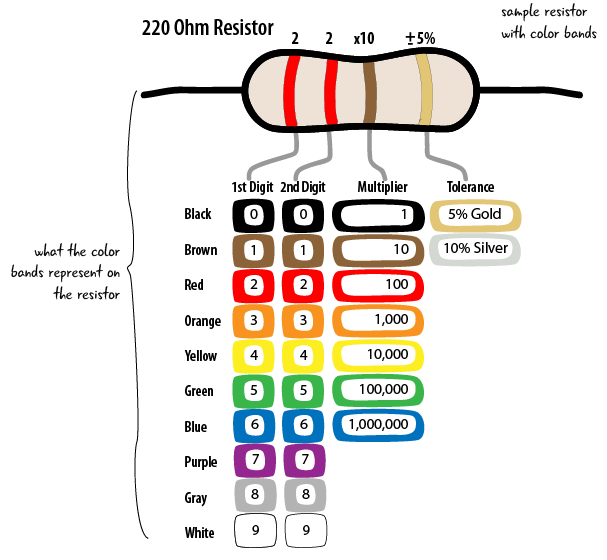
\includegraphics[width=.7\textwidth]{app-a-resistor-chart.png}
		\caption{The figure shows how to use the band pattern of a resistor to identify the resistor value and the tolerance.}
		\label{resistor-chart}
	\end{figure}
	\subsection*{Predicting Current and Voltage}
	\label{predict}
	\subsubsection*{Predicting Current}
	Follow the following steps to arrive at your predicted value for current.
	\begin{enumerate}
		\item First, use the loop rule and the node rule to set up and solve a system of equations to find the current through each resistor.
		\item Finding the nominal value for your predicted current is not too difficult: finding the uncertainty associated with this value is in general more challenging. The sources of uncertainty in your current calculation are the uncertainty in the emf of the battery and the tolerances of the resistors. These uncertainties combine in complicated ways to produce the overall uncertainty of the predicted current.
		
		We will use Python and the third party \href{https://pythonhosted.org/uncertainties/}{\texttt{uncertainties}} module to do this for us. To calculate the nominal value and uncertainty of your predicted current:
		\begin{enumerate}
			\item We will essentially be using Python as our calculator. Create variables to store the values of the battery emf and all of the resistors, and then perform the appropriate mathematical operation to obtain your predicted current.
			
			Instead of using normal \texttt{floats} for your variables above, you will use a special data type defined in the \texttt{uncerainties} package. Declare each variable using the \texttt{ufloat} function which accepts two arguments: the nominal value, and the uncertainty. So if your battery emf measurement had a mean of 8.76 V and a standard deviation of 0.14 V, you could declare a variable like:\\ 
			\begin{center}
			\texttt{batt\_emf=ufloat(8.76,0.14)}
			\end{center}
			Similarly, if your resistor has a resistance of 220 $\Omega$ and a tolerance of 10\%, you could create a resistance variable:\\
			\begin{center}
				\texttt{r1=ufloat(220, 220 * 0.1)}
			\end{center}
		\end{enumerate}
	
		The result of the \texttt{ufloat} function is not a normal \texttt{float} variable, but a special data type (called \texttt{uncertainties.core.Variable}) which gives you access to both the nominal value and the uncertainty of the variable. For instance, if you type \texttt{print(batt\_emf.nominal\_value)}, it will print 8.76. \texttt{batt\_emf.std\_dev} tells you the uncertainty.
		
		Once you have created variables in this way for every resistor and battery in your circuit, you can use these variables as you normally would in any other calculation. The key is that when you perform mathematical operations with these variables, the result will \textit{also} be a variable of the same data type. Therefore, you could run the code\\
		\begin{center}
			\texttt{ i\_predicted = batt\_emf / r1}
		\end{center}
	And then you can access the propagated uncertainty using the \texttt{i\_predicted} variable:\\
	\begin{center}
		\texttt{print("Predicted current= ", i\_predicted.nominal\_value)}\\
		\texttt{print("Uncertainty in predicted current= ", i\_predicted.std\_dev)}\
	\end{center}
	\end{enumerate}
	\subsubsection*{Predicting Voltage}
	Once you have your predicted current through each resistor, your predicted voltage is given by Ohm's Law: $\Delta V=IR$. Note that both $I$ and $R$ have uncertainties associated with them, so your predicted $V$ will also have such an uncertainty. You can use the \texttt{uncertainties} module to calculate these values, as described in the previous section.
	
	\subsection*{Measuring Current and Voltage}
	\label{measure}
	\subsubsection*{Measuring Current}
	To measure current:
	\begin{enumerate}
		\item Connect the multimeter in \textbf{series} with the circuit element whose current you want to measure. Be sure that conventional current flows \textit{into} the port labeled \texttt{A} and out of the port labeled \texttt{COM}. Do not connect the battery yet. Have your instructor check that your circuit is properly connected.
		\item Once your instructor has approved your circuit, connect the battery to apply power to the circuit.
		\item \textit{After} connecting your circuit, press the \texttt{DC I} button on the multimeter (this will refresh the statistics) 
		\item The multimeter takes measurements multiple times per second and tracks the mean and standard deviation. At the bottom of the multimeter screen, you can see this information along with a few other quantities. 
		
		Wait a few seconds while the multimeter accumulates data (wait until the \texttt{counts} quantity is at least 20 or so) and then record the mean and standard deviation \textit{before} disconnecting your circuit. 
	\end{enumerate}
	\subsubsection*{Measuring Voltage}
	To measure voltage:
	\begin{enumerate}
	\item Connect the multimeter in \textbf{parallel} with the circuit element whose voltage you want to measure. To measure positive voltage, the voltage read at the ``V'' port should be higher than the voltage at the ``COM'' port.  Do not connect the battery yet. 
	\item Connect the battery to apply power to the circuit.
	\item \textit{After} connecting your circuit, press the \texttt{DC V} button on the multimeter (this will refresh the statistics) 
	\item The multimeter takes measurements multiple times per second and tracks the mean and standard deviation. At the bottom of the multimeter screen, you can see this information along with a few other quantities. 
	
	Wait a few seconds while the multimeter accumulates data (wait until the \texttt{counts} quantity is at least 20 or so) and then record the mean and standard deviation \textit{before} disconnecting your circuit. 
	\end{enumerate}
\end{document}
